\section*{Introducción}
En esta práctica, se utilizó la herramienta Mockaroo para la generación de datos ficticios con el fin de poblar una base de datos de Juegos Olímpicos. Mockaroo es una herramienta en línea que permite generar datos de prueba de manera rápida y sencilla, lo cual es útil para realizar pruebas y desarrollos en bases de datos.

\section*{Generación de Datos con Mockaroo}
Para la generación de datos, se siguieron los siguientes pasos:
\begin{enumerate}
    \item Se accedió al sitio web de Mockaroo (\url{https://mockaroo.com/}).
    \item Revisamos la documentación de esta herramienta para entender su funcionamiento y hacer uso de ella.
    \item Entonces despues vimos el esquema de la base de datos para así ver que tablas se iban a poblar y que campos se iban a utilizar de las mismas.
    \begin{itemize}
        \item \textbf{Tabla Países}:
        \begin{itemize}
            \item \textbf{NombrePais}: Tipo de dato varchar(50).
        \end{itemize}
        \item \textbf{Tabla Medallero}:
        \begin{itemize}
            \item \textbf{IDMedallero}: Tipo de dato serial.
            \item \textbf{NombrePais}: Tipo de dato varchar(50).
        \end{itemize}
        \item \textbf{Tabla Concursa}:
        \begin{itemize}
            \item \textbf{IDAtleta}: Tipo de dato int.
            \item \textbf{IDEvento}: Tipo de dato int.
        \end{itemize}
        \item \textbf{Tabla Disciplinas}:
        \begin{itemize}
            \item \textbf{IDDisciplina}: Tipo de dato serial.
            \item \textbf{NombreDisciplina}: Tipo de dato varchar(50).
            \item \textbf{Categoria}: Tipo de dato varchar(50).
        \end{itemize}
        \item \textbf{Tabla Localidades}:
        \begin{itemize}
            \item \textbf{NombreLocalidad}: Tipo de dato varchar(50).
            \item \textbf{IDDisciplina}: Tipo de dato int.
            \item \textbf{Calle}: Tipo de dato varchar(50).
            \item \textbf{Numero}: Tipo de dato int.
            \item \textbf{Ciudad}: Tipo de dato varchar(50).
            \item \textbf{Pais}: Tipo de dato varchar(50).
            \item \textbf{Aforo}: Tipo de dato int.
            \item \textbf{Tipo}: Tipo de dato varchar(50).
        \end{itemize}
        \item \textbf{Tabla Eventos}:
        \begin{itemize}
            \item \textbf{IDEvento}: Tipo de dato serial.
            \item \textbf{NombreLocalidad}: Tipo de dato varchar(50).
            \item \textbf{IDDisciplina}: Tipo de dato int.
            \item \textbf{DuracionMax}: Tipo de dato int.
            \item \textbf{Precio}: Tipo de dato int.
            \item \textbf{FechaEvento}: Tipo de dato date.
            \item \textbf{Fase}: Tipo de dato int.
        \end{itemize}
        \item \textbf{Tabla Entrenadores}:
        \begin{itemize}
            \item \textbf{IDEntrenador}: Tipo de dato serial.
            \item \textbf{IDDisciplina}: Tipo de dato int.
            \item \textbf{Nombre}: Tipo de dato varchar(50).
            \item \textbf{PrimerApellido}: Tipo de dato varchar(50).
            \item \textbf{SegundoApellido}: Tipo de dato varchar(50).
            \item \textbf{FechaNacimiento}: Tipo de dato date.
            \item \textbf{Nacionalidad}: Tipo de dato varchar(50).
            \item \textbf{Genero}: Tipo de dato char(1).
        \end{itemize}
        \item \textbf{Tabla Atletas}:
        \begin{itemize}
            \item \textbf{IDAtleta}: Tipo de dato serial.
            \item \textbf{NombrePais}: Tipo de dato varchar(50).
            \item \textbf{IDEntrenador}: Tipo de dato int.
            \item \textbf{Temporada}: Tipo de dato date.
            \item \textbf{Nombre}: Tipo de dato varchar(50).
            \item \textbf{PrimerApellido}: Tipo de dato varchar(50).
            \item \textbf{SegundoApellido}: Tipo de dato varchar(50).
            \item \textbf{FechaNacimiento}: Tipo de dato date.
            \item \textbf{Nacionalidad}: Tipo de dato varchar(50).
            \item \textbf{Genero}: Tipo de dato char(1).
        \end{itemize}
        \item \textbf{Tabla CorreoAtleta}:
        \begin{itemize}
            \item \textbf{IDCorreo}: Tipo de dato varchar(50).
            \item \textbf{IDAtleta}: Tipo de dato int.
        \end{itemize}
        \item \textbf{Tabla Patrocinadores}:
        \begin{itemize}
            \item \textbf{NombrePatrocinador}: Tipo de dato varchar(50). \\
        \end{itemize}
        \textbf{(Nótese que aquí solamente se muestran algunos tipos de datos en sus respectivas tablas y no se muestran todas las tablas del model de la base de datos porque es a manera de ejemplo ...)} 
    \end{itemize}
    \item Mas tarde se configuraron los campos necesarios para cada tabla de la base de datos y así poder poblar nuestra BD. \\
    
    A continuación, se muestran algunas de configuraciones utilizadas para la generación de tuplas dentro de nuestra base de datos, para mas tarde exportar dichas dichas tuplas en formato SQL y crear el archivo DML.sql: \\
    
    
    \begin{figure}[h!]
        \centering
        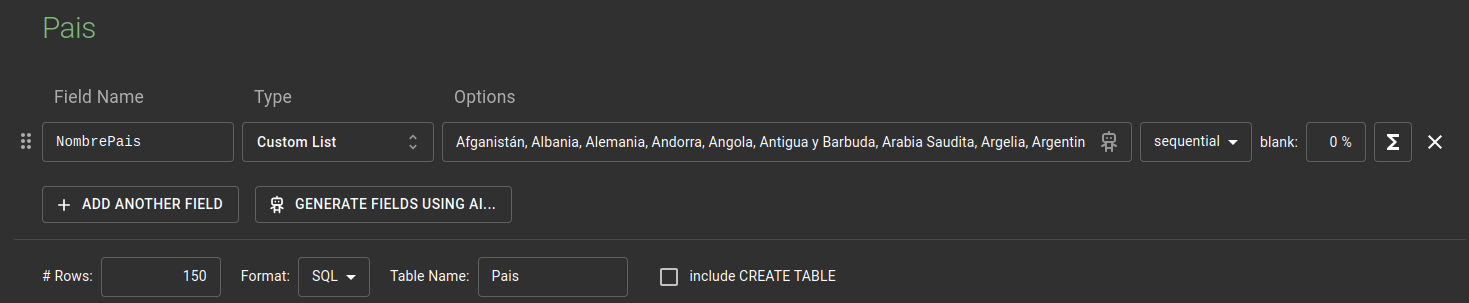
\includegraphics[width=1.1\textwidth]{../resources/Mockaroo/Pais.png} \\
    \end{figure}

    \newpage
    \begin{figure}[h!]
        \centering
        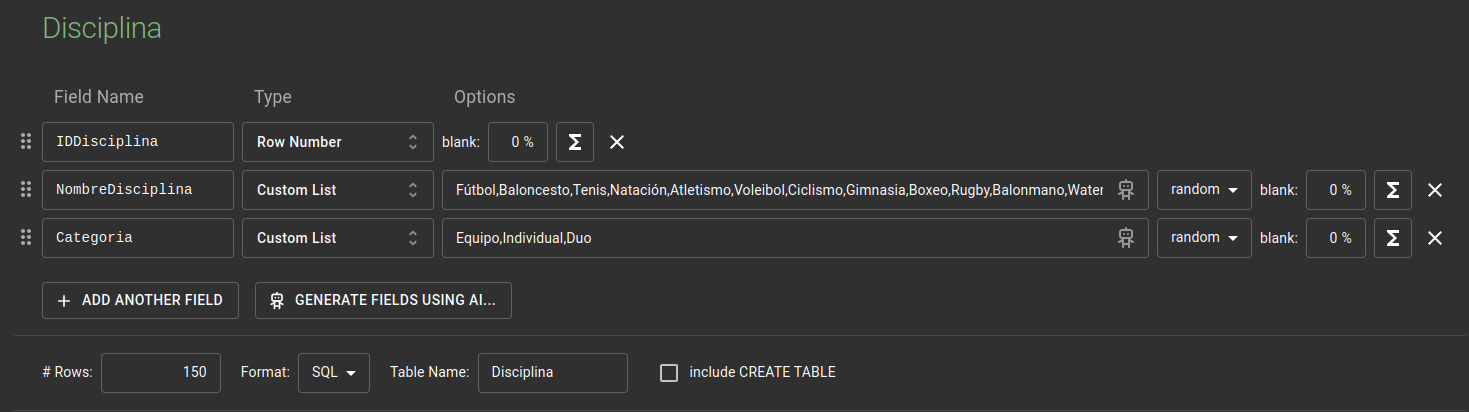
\includegraphics[width=1.1\textwidth]{../resources/Mockaroo/Disciplina.png} \\
    \end{figure}

    \begin{figure}[h!]
        \centering
        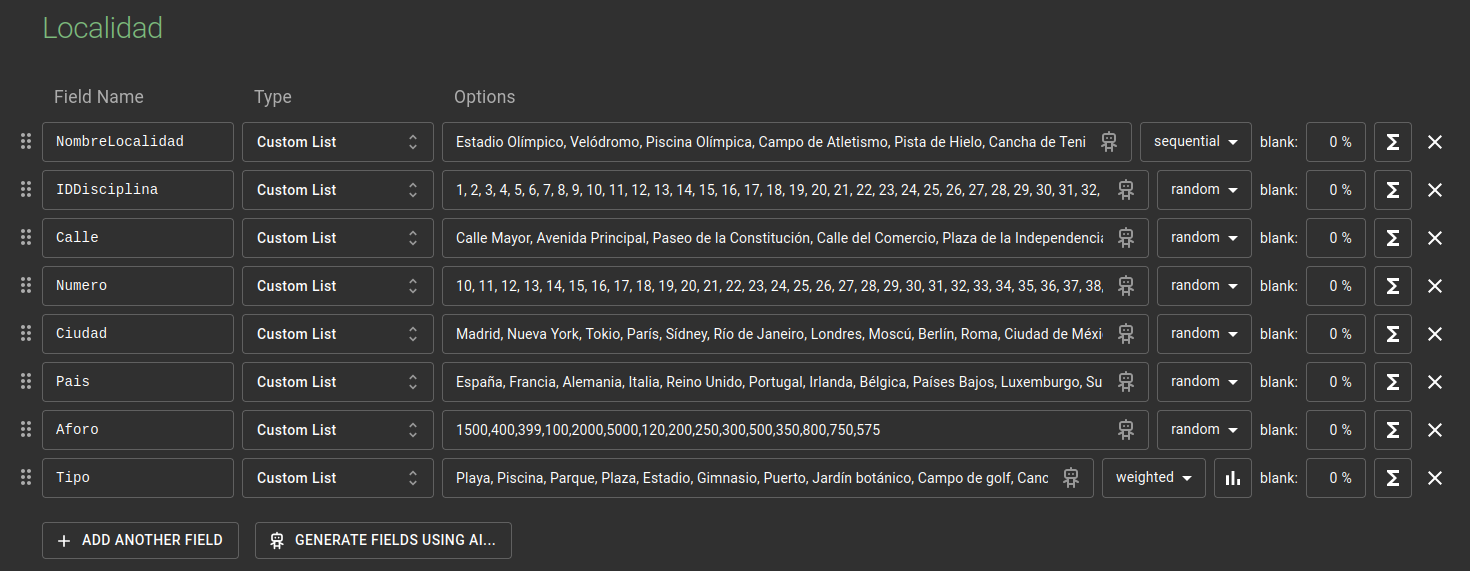
\includegraphics[width=1.1\textwidth]{../resources/Mockaroo/Localidad.png} \\
    \end{figure}

    \begin{figure}[h!]
        \centering
        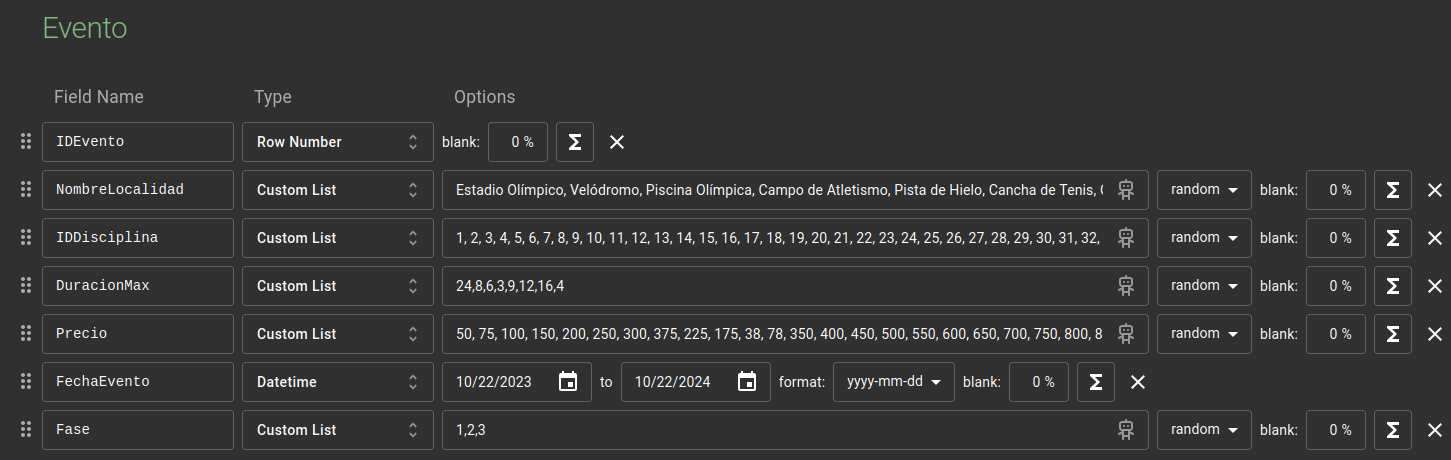
\includegraphics[width=1.1\textwidth]{../resources/Mockaroo/Evento.png} \\
    \end{figure}

    \begin{figure}[h!]
        \centering
        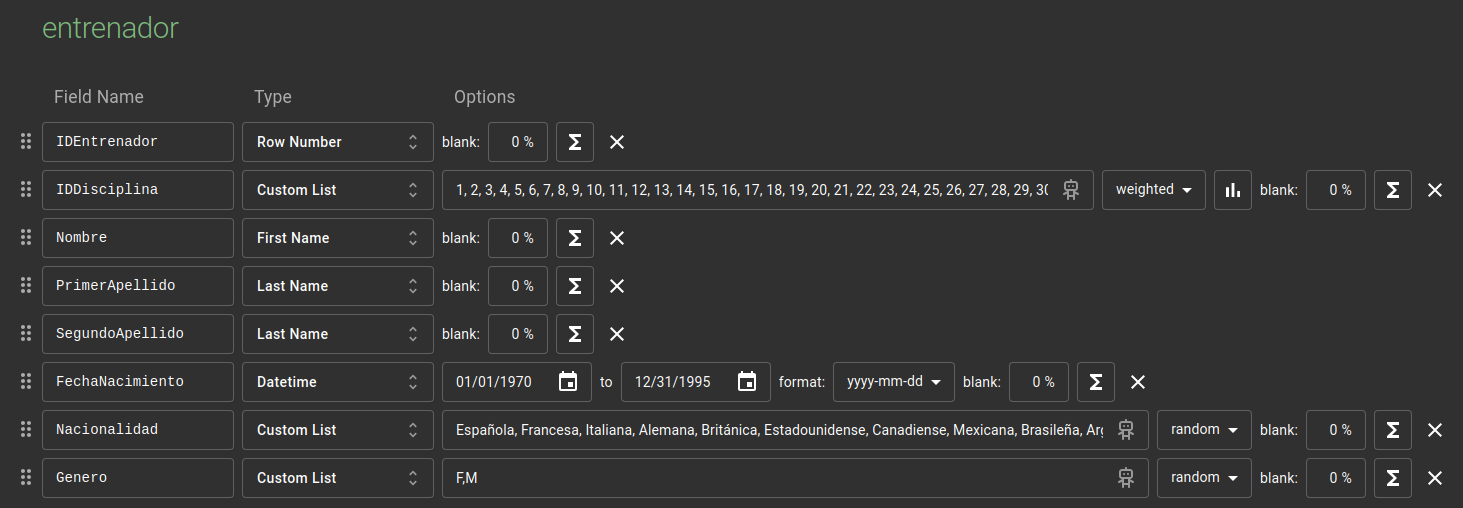
\includegraphics[width=1.1\textwidth]{../resources/Mockaroo/Entrenador.png} \\
    \end{figure}

    \newpage
    \begin{figure}[h!]
        \centering
        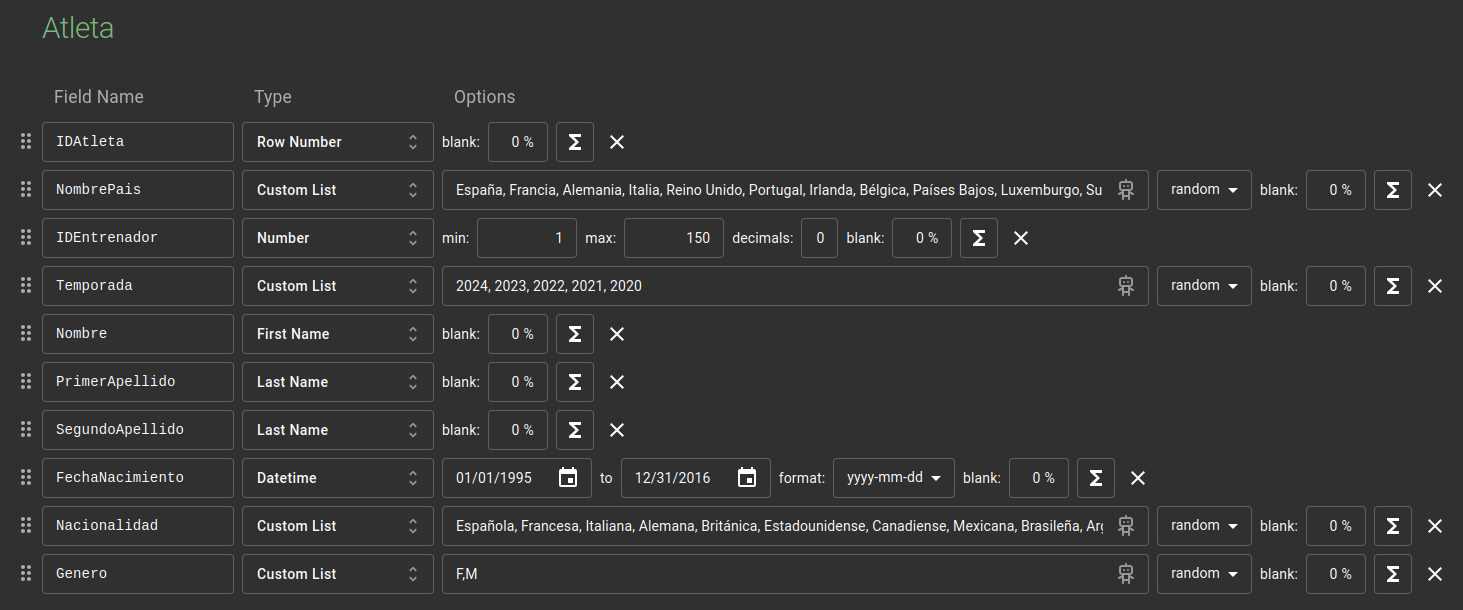
\includegraphics[width=1.1\textwidth]{../resources/Mockaroo/Atleta.png} \\
    \end{figure}

    \begin{figure}[h!]
        \centering
        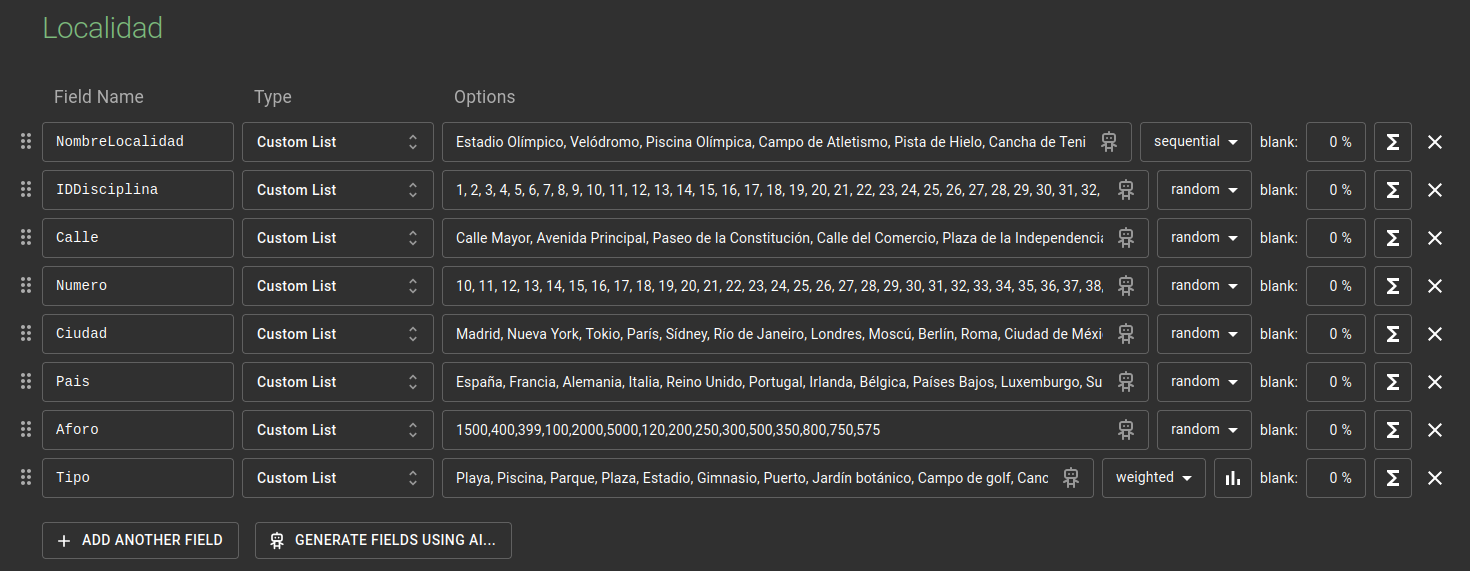
\includegraphics[width=1.1\textwidth]{../resources/Mockaroo/Localidad.png} \\
    \end{figure}

    \item Se generaron los datos y se descargaron en formato SQL. \\
    
    \textit{Ej: Tuplas tabla Evento} \\
    \begin{figure}[h!]
        \centering
        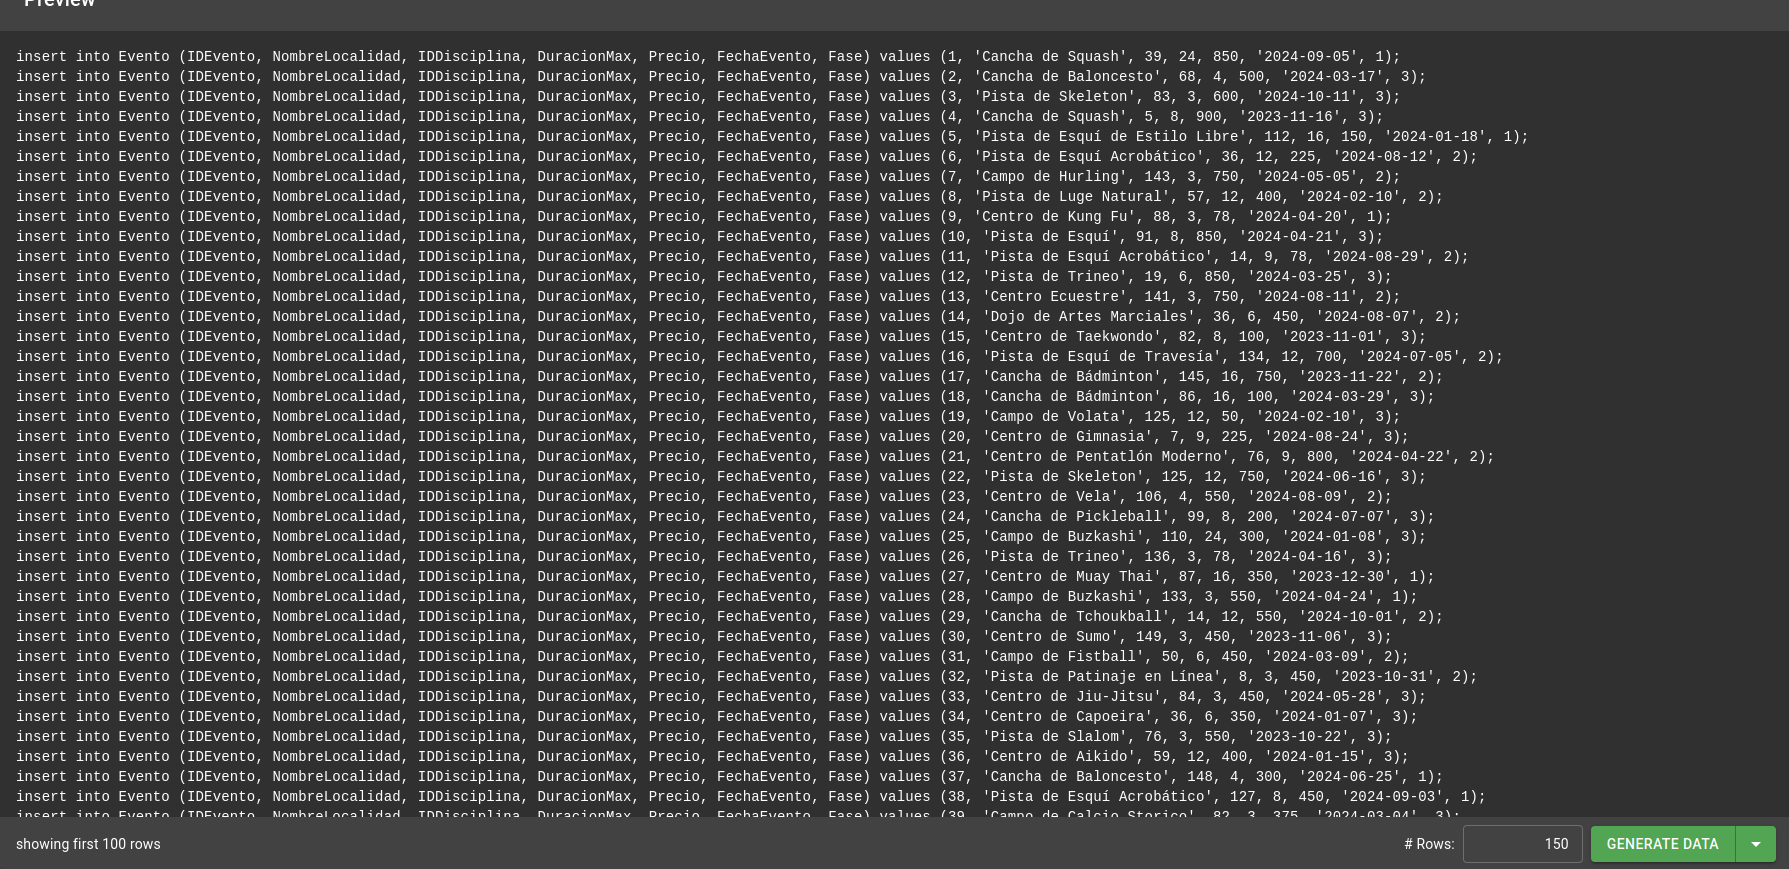
\includegraphics[width=1.1\textwidth]{../resources/Mockaroo/Ej_Evento.png} \\
    \end{figure}
\end{enumerate}


\section*{Carga de Datos en la Base de Datos}

Una vez generadas las tuplas, se procedió a crear el archivo DML.sql donde se coloco el código SQL generado por Mockaroo para cada tabla de la base de datos. \\

A continuación, se muestran algunos ejemplos de tuplas generadas por Mockaroo y el código SQL correspondiente para insertar los datos en la base de datos. \\


\begin{verbatim}
-- Insertar datos en la tabla Países
insert into Pais (NombrePais) values ('Afganistán');
insert into Pais (NombrePais) values ('Albania');
\end{verbatim}

\begin{verbatim}
-- Insertar datos en la tabla Disciplinas
insert into Disciplina (IDDisciplina, NombreDisciplina, Categoria) values 
(1, 'Fútbol', 'Equipo');
insert into Disciplina (IDDisciplina, NombreDisciplina, Categoria) values 
(2, 'Baloncesto', 'Individual');
\end{verbatim}

\begin{verbatim}
-- Insertar datos en la tabla Localidades
insert into Localidad (NombreLocalidad, IDDisciplina, Calle, Numero, Ciudad, Pais, Aforo, Tipo) 
values ('Estadio Olímpico', 111, 'Plaza de la República', 74, 'París', 'Túnez', 5000, 'Granja');
\end{verbatim}

\begin{verbatim}
-- Insertar datos en la tabla Eventos
insert into Evento (IDEvento, NombreLocalidad, IDDisciplina, DuracionMax, 
Precio, FechaEvento, Fase) values (1, 'Centro de Esgrima', 82, 16, 175, '2024-02-24', 2);
\end{verbatim}

\begin{verbatim}
-- Insertar datos en la tabla Entrenadores
insert into Entrenador (IDEntrenador, IDDisciplina, Nombre, PrimerApellido, SegundoApellido, 
FechaNacimiento, Nacionalidad, Genero)values 
(1, 17, 'Mordecai', 'Bodemeaid', 'Ratnage', '1979-11-05', 'Malasia', 'M');
\end{verbatim}

\begin{verbatim}
-- Insertar datos en la tabla Atletas
insert into Atleta (IDAtleta, NombrePais, IDEntrenador, Temporada, Nombre, PrimerApellido,
SegundoApellido, FechaNacimiento, Nacionalidad, Genero) values (1, 'República Dominicana', 
13, 2021, 'Justina', 'Halpeine', 'Lothlorien', '2001-05-05', 'Kazaja', 'M');
\end{verbatim}

\begin{verbatim}
-- Insertar datos en la tabla CorreoAtleta
insert into CorreoAtleta (IDCorreo, IDAtleta) values ('john.doe@gmail.com', 79);
insert into CorreoAtleta (IDCorreo, IDAtleta) values ('jane.smith@yahoo.com', 16);
\end{verbatim}

\begin{verbatim}
-- Insertar datos en la tabla Patrocinadores
insert into Patrocinador (NombrePatrocinador) values ('Coca-Cola');
insert into Patrocinador (NombrePatrocinador) values ('Pepsi');
\end{verbatim}


En conclusión, el uso de Mockaroo en esta práctica facilitó la generación de datos ficticios para poblar la base de datos relacional de Juegos Olímpicos en la que hemos estado trabajando. Esta herramienta nos permitió generar datos de manera rápida y sencilla, y además, los datos generados se cargaron en la base utilizando instrucciones SQL, cumpliendo con las restricciones de diseño de la base de datos.
